\documentclass[11pt,a4paper]{article}
\usepackage[utf8]{inputenc}
\usepackage[T1]{fontenc}
\usepackage{times}
\renewcommand{\figurename}{Figura}
\renewcommand{\tablename}{Tabla}
\renewcommand{\refname}{Referencias}
\renewcommand{\abstractname}{Resumen}
\usepackage[margin=2.5cm]{geometry}
\usepackage{amsmath,amssymb}
\usepackage{graphicx}
\usepackage{booktabs}
\usepackage{caption}
\usepackage[numbers,sort&compress]{natbib}
\usepackage{hyperref}
\usepackage{enumitem}
\setlength{\parindent}{1.2em}
\setlength{\parskip}{4pt}
\captionsetup{font=small,labelfont=bf}
\newcommand{\CODIGO}{\url{https://github.com/jessicaromero-ctrl/algoritmos-evolutivos/tree/main/Actividades/Corte_03/Actividad_07_Flowshop_Energia}}

\title{\textbf{Programación de un flow shop de permutación con energía mediante NSGA-II:\\comparación de operadores de cruce en una línea de envasado}}
\author{Jessica Melani Romero Lora\\
\small Matrícula 25322116 \\
\small Maestría en Inteligencia Artificial, Universidad Politécnica Metropolitana de Hidalgo\\
\small Materia: Algoritmos Evolutivos \quad Docente: Dr. Jaime Aguilar Ortiz}
\date{Noviembre de 2026}

\begin{document}
\maketitle

\begin{abstract}
\noindent Este trabajo aplica optimización multiobjetivo a la secuenciación de lotes en un \emph{flow shop} de permutación con cuatro máquinas en serie y consumo de energía. Se consideran tres objetivos en conflicto: el tiempo total de terminación ($C_{\max}$), la tardanza ponderada y la energía consumida, que depende de la secuencia a través de los tiempos ociosos y de una política de apagado óptimo. Se compara NSGA-II con dos operadores de cruce para permutaciones (OX y PMX) frente a búsqueda aleatoria, con 30 semillas emparejadas. En una instancia de nueve lotes, el frente de Pareto exacto se obtuvo por enumeración de las $9!$ secuencias. NSGA-II recupera en promedio 23 y 24 de los 28 puntos exactos, con solo 1.7\,\% de las evaluaciones posibles; la búsqueda aleatoria recupera 0.4. En una instancia de 25 lotes, PMX supera a OX en distancia generacional invertida (0.036 frente a 0.058). Los resultados muestran que la secuencia de mínimo $C_{\max}$ tiene una tardanza más del doble que la de compromiso, y que la energía varía 2\,\% a lo largo del frente. El código, las pruebas y los resultados están disponibles en el repositorio citado.
\end{abstract}

\noindent\textbf{Palabras clave:} \emph{flow shop}, programación de la producción, NSGA-II, optimización multiobjetivo, energía, operadores de permutación.

\section{Introducción}
La programación de la producción decide en qué orden se procesan los lotes en los recursos disponibles. Una decisión de secuencia afecta de forma simultánea el tiempo de entrega, el cumplimiento de fechas, la utilización de máquinas y el consumo de energía. En las plantas de manufactura mexicanas, donde la presión de costos y la competencia por plazos de entrega son constantes, estas decisiones suelen tomarse con reglas de despacho sencillas, como la fecha de entrega más próxima, que atienden un criterio a la vez.

Este trabajo plantea la secuenciación como un problema multiobjetivo en un \emph{flow shop} de permutación con energía, inspirado en una línea de envasado de bebidas. El objetivo es obtener el conjunto de secuencias no dominadas y comparar el desempeño de un algoritmo evolutivo multiobjetivo frente a una búsqueda sin guía. La contribución es doble: una formulación con energía dependiente de la secuencia y una evaluación rigurosa contra el frente exacto en una instancia pequeña y contra un frente de referencia en una instancia mayor.

\section{Flow shop: objetivo y fundamentos}
\subsection{Definición y objetivo}
Un \emph{flow shop} es un sistema de producción en el que $n$ trabajos deben procesarse en $m$ máquinas, todas en la misma secuencia de operaciones: primero en la máquina 1, luego en la 2, y así sucesivamente. Cuando la secuencia de trabajos es la misma en todas las máquinas, el sistema se llama \emph{flow shop de permutación}. Ese es el caso aquí, y la decisión consiste en encontrar la permutación $\pi$ de los $n$ trabajos.

El objetivo clásico es minimizar el tiempo total de terminación, o \emph{makespan}, que es la terminación del último trabajo en la última máquina. En la práctica se añaden criterios de servicio, como la tardanza respecto a la fecha de entrega, y criterios de costo, como la energía. Como estos criterios entran en conflicto, el problema se resuelve mejor como búsqueda de un frente de Pareto, no como la minimización de una sola función.

\begin{figure}[t]
\centering
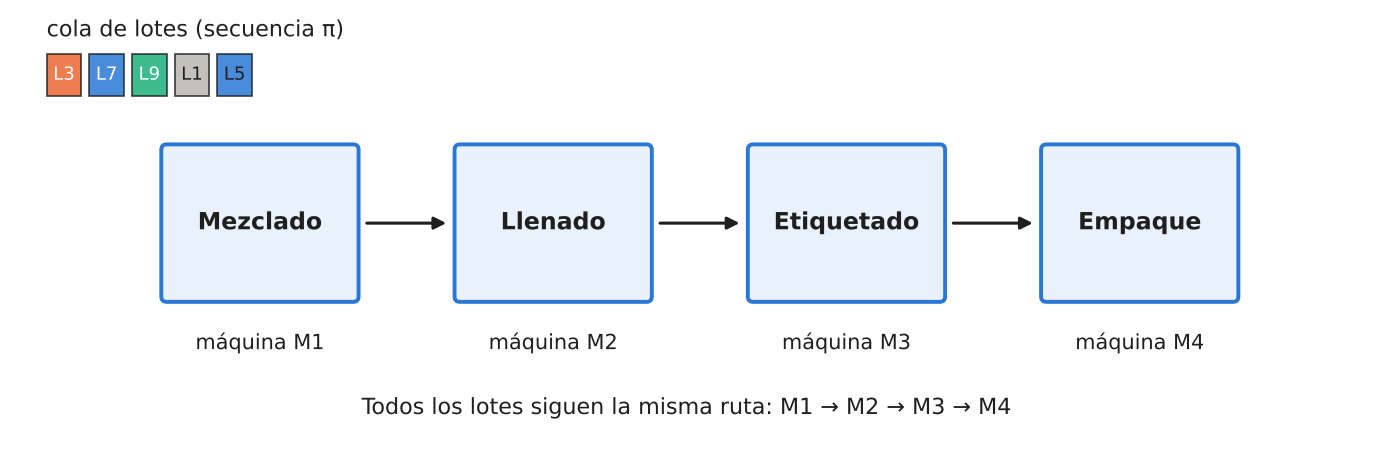
\includegraphics[width=0.92\linewidth]{../figuras/fig1_esquema_flowshop.png}
\caption{Esquema de un flow shop de permutación con cuatro máquinas en serie. Todos los lotes siguen la misma ruta; la decisión es el orden de la cola.}
\label{fig:esquema}
\end{figure}


\subsection{Notación y complejidad}
La clasificación de Graham et al.\ \cite{graham1979} describe un problema de secuenciación con la notación $\alpha|\beta|\gamma$. El problema estudiado es $F_m|\mathrm{perm}|\,\cdot$, con $m=4$ y criterios múltiples. Johnson \cite{johnson1954} resolvió de forma exacta el caso de dos máquinas, pero Garey et al.\ \cite{garey1976} demostraron que $F_m|\mathrm{perm}|C_{\max}$ es NP-difícil para $m\geq 3$. Por esa razón, en instancias de tamaño realista se usan heurísticas y metaheurísticas \cite{ruiz2007,pinedo2016}, y en este trabajo, un algoritmo evolutivo multiobjetivo.

\subsection{Relevancia industrial}
El \emph{flow shop} describe líneas de envasado, de ensamble en serie y de procesos por etapas, donde cada producto sigue la misma ruta. Su optimización reduce inventarios en proceso, acorta plazos de entrega y disminuye tiempos ociosos, lo que a su vez reduce consumo energético. Mouzon et al.\ \cite{mouzon2007} documentan que los tiempos ociosos de equipos encendidos representan una fracción relevante del consumo de energía en la manufactura, lo que justifica incluir la energía como objetivo de secuenciación.

\section{Mercados de producción y de consumo}
\subsection{Mercados de producción}
Los sectores que operan con líneas de flujo en México son los que más se benefician de la secuenciación multiobjetivo. Tres de ellos concentran el mayor peso económico. La \textbf{industria alimentaria y de bebidas} opera líneas de mezclado, llenado, etiquetado y empaque con fechas de entrega a distribuidores y con restricciones de vida útil. La \textbf{fabricación de equipo de transporte} organiza líneas de ensamble en serie con estaciones de soldadura, pintura y ensamble final. La \textbf{industria farmacéutica y de empaque} combina procesos de llenado y serialización con validaciones de calidad. En los tres casos, un cambio en la secuencia altera el cumplimiento de entregas y el consumo energético de las máquinas que esperan.

\subsection{Mercados de consumo}
Los productos que salen de estas líneas se venden principalmente en tres canales: el autoservicio y el comercio minorista de alimentos y bebidas en el mercado nacional, la distribución mayorista a restaurantes y servicios, y la exportación, en particular de componentes y vehículos hacia América del Norte. La puntualidad de las entregas es un criterio comercial directo en los dos primeros canales, porque una tardanza en un lote de bebidas implica faltantes en anaquel.

\section{Contexto actual de México}
Según el INEGI, la industria manufacturera generó 7.15 billones de pesos en el segundo trimestre de 2026, equivalentes al 20.5\,\% del PIB nominal \cite{inegi2026pib}. Dentro de la manufactura, la industria alimentaria aporta alrededor de una quinta parte del valor, y el equipo de transporte una proporción similar; ambos subsectores concentran cerca de 42\,\% del valor manufacturero. En la Encuesta Anual de la Industria Manufacturera de 2024, el equipo de transporte encabeza el valor de la producción con 32.6\,\% \cite{inegi2025eaim}.

Dos factores explican la relevancia actual del problema. El primero es el \emph{nearshoring}: la reubicación de cadenas productivas hacia México, que aumenta la demanda de capacidad y de planeación de líneas. Un reporte periodístico con datos del INEGI atribuye a la manufactura cerca de la mitad de la inversión extranjera directa \cite{mexicoindustry2026ied}. El segundo es la presión de costos. Las encuestas de gerentes de compras de S\&P Global reportaron contracción de la actividad manufacturera en marzo de 2026, asociada con la intensa presión de costos \cite{spglobal2026pmi}. En ese contexto, reducir tiempos ociosos y tardanzas sin nueva inversión en equipo es una palanca directa de competitividad.

\section{Despliegue comercial principal}
La solución propuesta se comercializa como un módulo de planeación y secuenciación para líneas en serie, que se integra con los sistemas de planeación de recursos empresariales (ERP) y de ejecución de manufactura (MES) existentes. El segmento inicial son medianas plantas de alimentos y bebidas con entre tres y seis líneas de envasado y necesidades de cumplimiento de entregas.

La propuesta de valor se mide en tres indicadores verificables: reducción de tardanza ponderada, reducción de consumo energético por lote y tiempo de respuesta ante cambios de pedido. El modelo de ingreso combina una licencia por línea, un servicio de implantación con piloto de dos a cuatro semanas en una línea real, y un contrato de soporte anual. El piloto es la pieza clave de la venta: permite comparar la secuencia actual de la planta con las soluciones del frente de Pareto y mostrar el compromiso entre entrega y energía con datos del propio cliente.

Como riesgos comerciales se identifican la calidad de los datos de tiempos de proceso, que deben medirse en planta, y la resistencia a cambiar reglas de despacho conocidas. Ambos se atienden con la fase de piloto y con una interfaz que muestra las alternativas de secuencia con su costo en términos de los tres objetivos.

\section{Modelo matemático}
Sea $J=\{1,\dots,n\}$ el conjunto de lotes y $M=\{1,\dots,m\}$ el de máquinas. El parámetro $p_{ji}$ es el tiempo de proceso del lote $j$ en la máquina $i$, $d_j$ su fecha de entrega y $w_j$ su peso de prioridad. Para una permutación $\pi$, la terminación y el inicio del lote en la posición $k$ en la máquina $i$ satisfacen la recurrencia:
\begin{equation}
C_{k,i}(\pi)=\max\{C_{k-1,i}(\pi),\,C_{k,i-1}(\pi)\}+p_{\pi(k),i},\qquad C_{0,i}=C_{k,0}=0,
\label{eq:recurrencia}
\end{equation}
con inicio $S_{k,i}(\pi)=C_{k,i}(\pi)-p_{\pi(k),i}$. Los tres objetivos se definen como:
\begin{align}
f_1(\pi) &= C_{\max}(\pi)=C_{n,m}(\pi), \label{eq:f1}\\
f_2(\pi) &= \sum_{k=1}^{n} w_{\pi(k)}\,\max\{0,\;C_{k,m}(\pi)-d_{\pi(k)}\}, \label{eq:f2}\\
f_3(\pi) &= \sum_{i=1}^{m} P_i^{\mathrm{act}}\frac{\sum_{k} p_{\pi(k),i}}{60}
  + \sum_{i=1}^{m}\sum_{k=2}^{n}\min\!\left\{P_i^{\mathrm{idle}}\,\frac{S_{k,i}(\pi)-C_{k-1,i}(\pi)}{60},\;E_i^{\mathrm{arr}}\right\}
  + \sum_{i=1}^{m}E_i^{\mathrm{arr}}. \label{eq:f3}
\end{align}
La energía $f_3$ está en kWh, con tiempos en minutos. El primer término es la energía en operación, constante para todas las secuencias. El segundo es la energía de los huecos ociosos: cada hueco consume potencia en espera o, si es más barato, la máquina se apaga y se reinicia con costo $E_i^{\mathrm{arr}}$. Este término depende de la secuencia, y por eso el consumo no es una función fija de $C_{\max}$. El tercer término es el arranque inicial.

El problema es:
\begin{equation}
\min_{\pi\in\Pi_n}\;\mathbf{f}(\pi)=\big(f_1(\pi),f_2(\pi),f_3(\pi)\big),
\label{eq:problema}
\end{equation}
donde $\Pi_n$ es el conjunto de las $n!$ permutaciones. Una solución $\pi$ domina a $\pi'$ si $f_q(\pi)\leq f_q(\pi')$ para todo $q$ y existe $q$ con desigualdad estricta. El conjunto de soluciones no dominadas es el frente de Pareto.

\section{Método: etapas}
El método se organiza en siete etapas.
\begin{enumerate}[leftmargin=2em]
\item \textbf{Instancia.} Se generan tiempos de proceso por máquina en intervalos realistas: mezclado de 10 a 25 min, llenado de 8 a 20 min, etiquetado de 5 a 12 min y empaque de 6 a 15 min por lote. Las fechas de entrega se toman entre el 35\,\% y el 95\,\% de una cota inferior del makespan, y los pesos en $\{1,2,3\}$.
\item \textbf{Frente exacto (instancia pequeña).} Para $n=9$ se evalúan las $9!=362\,880$ permutaciones en lotes vectorizados. El frente no dominado se extrae con un barrido lexicográfico, que es exacto porque ningún punto posterior puede dominar a uno anterior.
\item \textbf{Representación.} Cada individuo es una permutación de $\{0,\dots,n-1\}$.
\item \textbf{Inicialización y evaluación.} Población inicial de 60 permutaciones aleatorias; evaluación por la recurrencia de la ecuación~(1).
\item \textbf{Selección, cruce y mutación.} Torneo binario según rango de no dominancia y distancia de aglomeración. Cruce con probabilidad 0.9: OX \cite{davis1985}, que copia un segmento de un padre y completa con el orden relativo del otro, o PMX \cite{goldberg1985}, que copia un segmento y repara conflictos por correspondencia. Mutación por intercambio de dos posiciones con probabilidad 0.3 por hijo.
\item \textbf{Reemplazo.} Selección $\mu+\lambda$ con ordenamiento no dominado de NSGA-II \cite{deb2002}.
\item \textbf{Paro y comparación.} Presupuesto fijo de evaluaciones: 6\,000 en la instancia pequeña y 20\,000 en la grande. Treinta semillas emparejadas por algoritmo. Las métricas son el hipervolumen (referencia $1.1$ en espacio normalizado), la distancia generacional invertida (IGD) y el número de puntos exactos recuperados \cite{zitzler1999,coello2007}.
\end{enumerate}

\section{Implementación y código}
El código está en Python, con NumPy para la evaluación por lotes y SciPy para las pruebas estadísticas. Se organiza en tres módulos: \texttt{flowshop\_modelo.py} (instancias, evaluación, frente exacto), \texttt{flowshop\_moea.py} (NSGA-II, operadores OX y PMX, búsqueda aleatoria, métricas) y \texttt{experimento.py} (protocolo y estadística), más \texttt{figuras.py} y nueve pruebas automatizadas. Las pruebas verifican el makespan y la energía contra cálculos independientes, la validez de los operadores, la coincidencia del ordenamiento no dominado con fuerza bruta y la reproducibilidad. El código completo está disponible en \CODIGO.

Dos decisiones de implementación merecen mención. Primero, el conteo de dominancia del ordenamiento no dominado fue corregido tras una prueba de contraste contra fuerza bruta: en una versión inicial contaba las soluciones dominadas en lugar de las que dominan, y el algoritmo resultante era peor que la búsqueda aleatoria. Segundo, la normalización de las métricas de la instancia grande se calcula con el rango de todas las soluciones evaluadas, para que ningún método quede fuera de la caja de referencia del hipervolumen.

\section{Resultados}
\subsection{Instancia pequeña: frente exacto}
El frente exacto de la instancia de nueve lotes tiene 28 puntos no dominados. La Tabla~1 muestra cuatro secuencias representativas. La secuencia de mínimo $C_{\max}$ (174 min) tiene una tardanza ponderada de 366, más de seis veces la de mínima tardanza. La secuencia de compromiso, la más cercana al punto ideal en el espacio normalizado, reduce la tardanza a 161 con un incremento de un minuto en $C_{\max}$ y de 0.1\,kWh en energía. Esta secuencia es la de mayor interés para el decisor.

\begin{table}[t]
\centering
\caption{Puntos representativos del frente exacto (instancia de 9 lotes).}
\label{tab:decision}
\begin{tabular}{@{}lrrrl@{}}
\toprule
Criterio & $C_{\max}$ (min) & Tardanza & Energía (kWh) & Secuencia \\
\midrule
Mínimo $C_{\max}$ & 174 & 366 & 319.22 & T3 T7 T9 T6 T8 T4 T1 T5 T2 \\
Mínima tardanza & 189 & 57 & 324.38 & T3 T7 T2 T5 T6 T1 T8 T4 T9 \\
Mínima energía & 175 & 374 & 318.03 & T3 T4 T8 T5 T9 T6 T7 T1 T2 \\
Compromiso & 175 & 161 & 319.12 & T3 T7 T5 T9 T6 T8 T4 T1 T2 \\
\bottomrule
\end{tabular}
\end{table}

La Figura~2 proyecta el frente exacto frente a una muestra aleatoria. La energía varía 2.0\,\% a lo largo del frente, es decir, 6.3\,kWh entre el extremo de mínima energía y el de mínima tardanza. Esta variación es moderada porque la energía en operación domina el consumo. Además, la secuencia de mínima energía tiene una tardanza 2.3 veces mayor que la de compromiso, lo que confirma el conflicto entre energía y cumplimiento. La Figura~3 muestra cómo las dos secuencias extremas generan patrones de huecos distintos en las máquinas de empaque y etiquetado.

\begin{figure}[t]
\centering
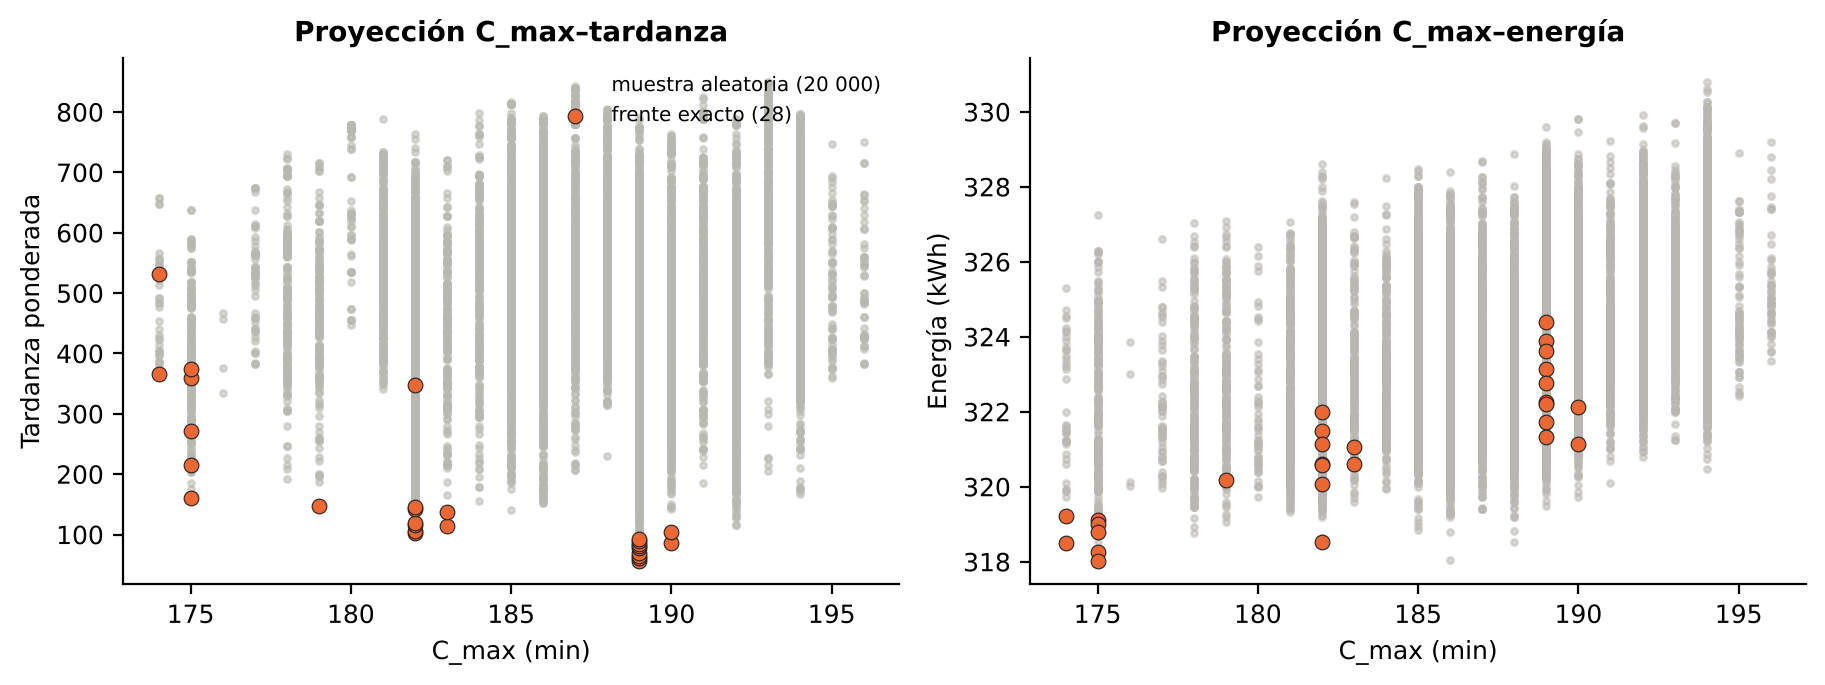
\includegraphics[width=\linewidth]{../figuras/fig3_frente_exacto.png}
\caption{Proyecciones del frente de Pareto exacto (28 puntos, en naranja) frente a una muestra aleatoria de 20\,000 secuencias (en gris).}
\label{fig:frente}
\end{figure}

\begin{figure}[t]
\centering
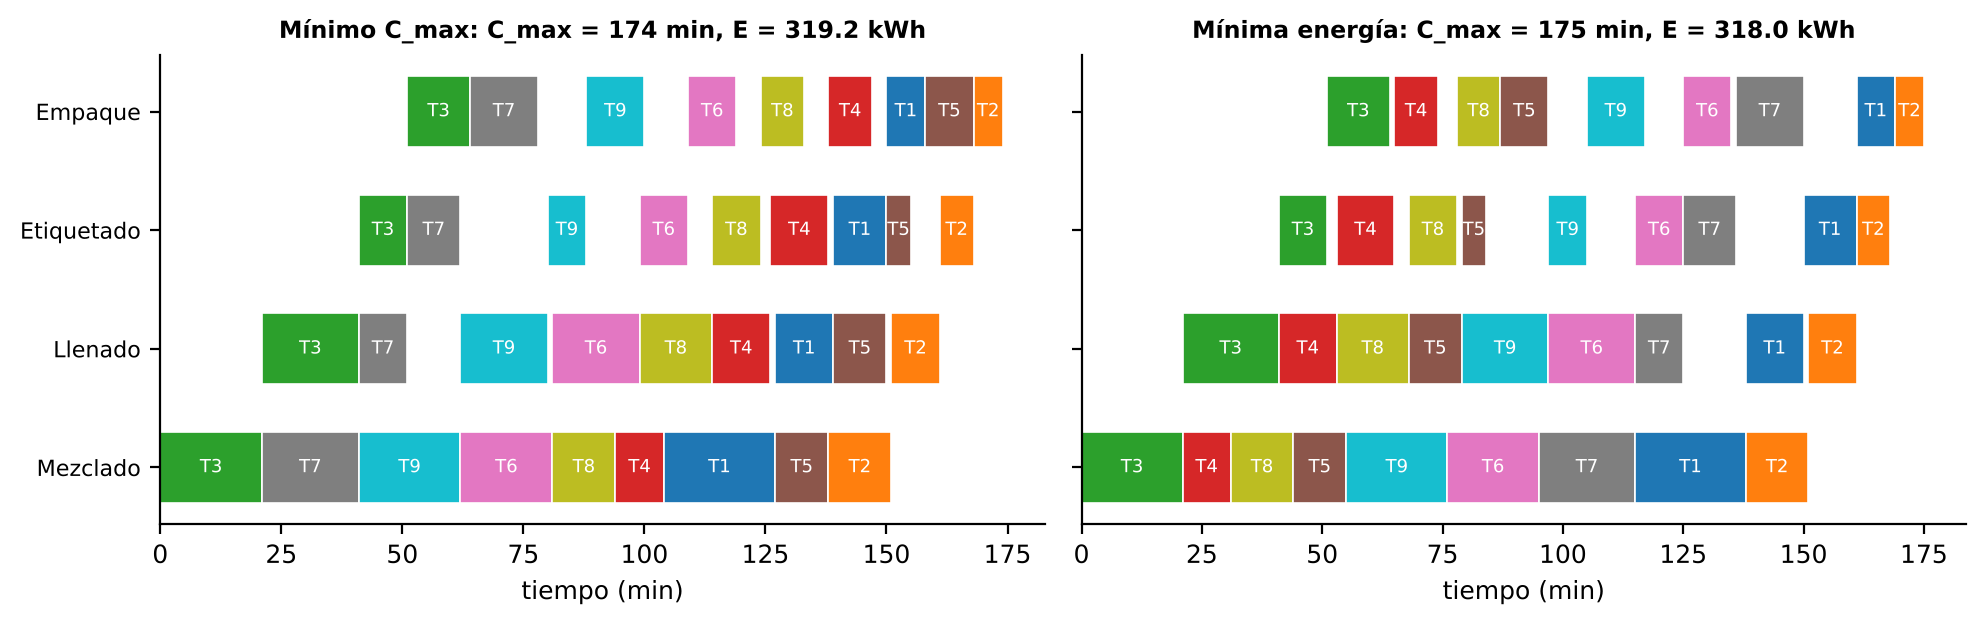
\includegraphics[width=\linewidth]{../figuras/fig2_gantt.png}
\caption{Diagramas de Gantt de las secuencias de mínimo $C_{\max}$ (izquierda) y de mínima energía (derecha). Los huecos en las máquinas finales determinan el consumo ocioso.}
\label{fig:gantt}
\end{figure}

\subsection{Comparación de algoritmos}
La Tabla~2 resume las métricas de los tres métodos. Con 6\,000 evaluaciones, equivalentes al 1.7\,\% del espacio, NSGA-II con OX recupera en promedio 23.0 puntos exactos y con PMX, 24.4. La búsqueda aleatoria recupera 0.4. El hipervolumen exacto del frente es 1.209; NSGA-II alcanza 1.196 y 1.196 respectivamente, es decir, 99\,\% de la referencia.

\begin{table}[t]
\centering
\caption{Métricas medianas por algoritmo. Instancia A: frente exacto de 28 puntos; instancia B: referencia de 79 puntos. Treinta semillas.}
\label{tab:comparacion}
\begin{tabular}{@{}llrrrr@{}}
\toprule
Instancia & Algoritmo & HV & IGD & IGD (RIQ) & Recuperados \\
\midrule
A ($n=9$) & NSGA-II (OX) & 1.1956 & 0.0145 & 0.0127--0.0156 & 23.0 \\
A ($n=9$) & NSGA-II (PMX) & 1.1963 & 0.0117 & 0.0113--0.0137 & 24.4 \\
A ($n=9$) & Aleatoria & 1.1159 & 0.0704 & 0.0644--0.0760 & 0.4 \\
B ($n=25$) & NSGA-II (OX) & 1.2384 & 0.0584 & 0.0486--0.0625 & --- \\
B ($n=25$) & NSGA-II (PMX) & 1.2713 & 0.0364 & 0.0333--0.0405 & --- \\
B ($n=25$) & Aleatoria & 0.9275 & 0.2495 & 0.2405--0.2603 & --- \\
\bottomrule
\end{tabular}
\end{table}

Las pruebas de Wilcoxon emparejadas por semilla, con corrección de Holm, dan los siguientes resultados. En la instancia A, PMX recupera más puntos exactos que OX (A12 = 0.74 a favor de PMX; $p_{\mathrm{Holm}}=0.002$) y obtiene menor IGD ($p_{\mathrm{Holm}}=0.005$); la diferencia de hipervolumen no es significativa ($p_{\mathrm{Holm}}=0.152$). En la instancia B, PMX supera a OX en IGD e hipervolumen ($p_{\mathrm{Holm}}<0.001$ en ambos), con un tamaño de efecto A12 de 0.96 en IGD. Frente a la búsqueda aleatoria, los dos operadores de NSGA-II son superiores en todas las métricas con A12 = 1 y $p_{\mathrm{Holm}}<0.001$. La Figura~4 muestra las distribuciones.

\begin{figure}[t]
\centering
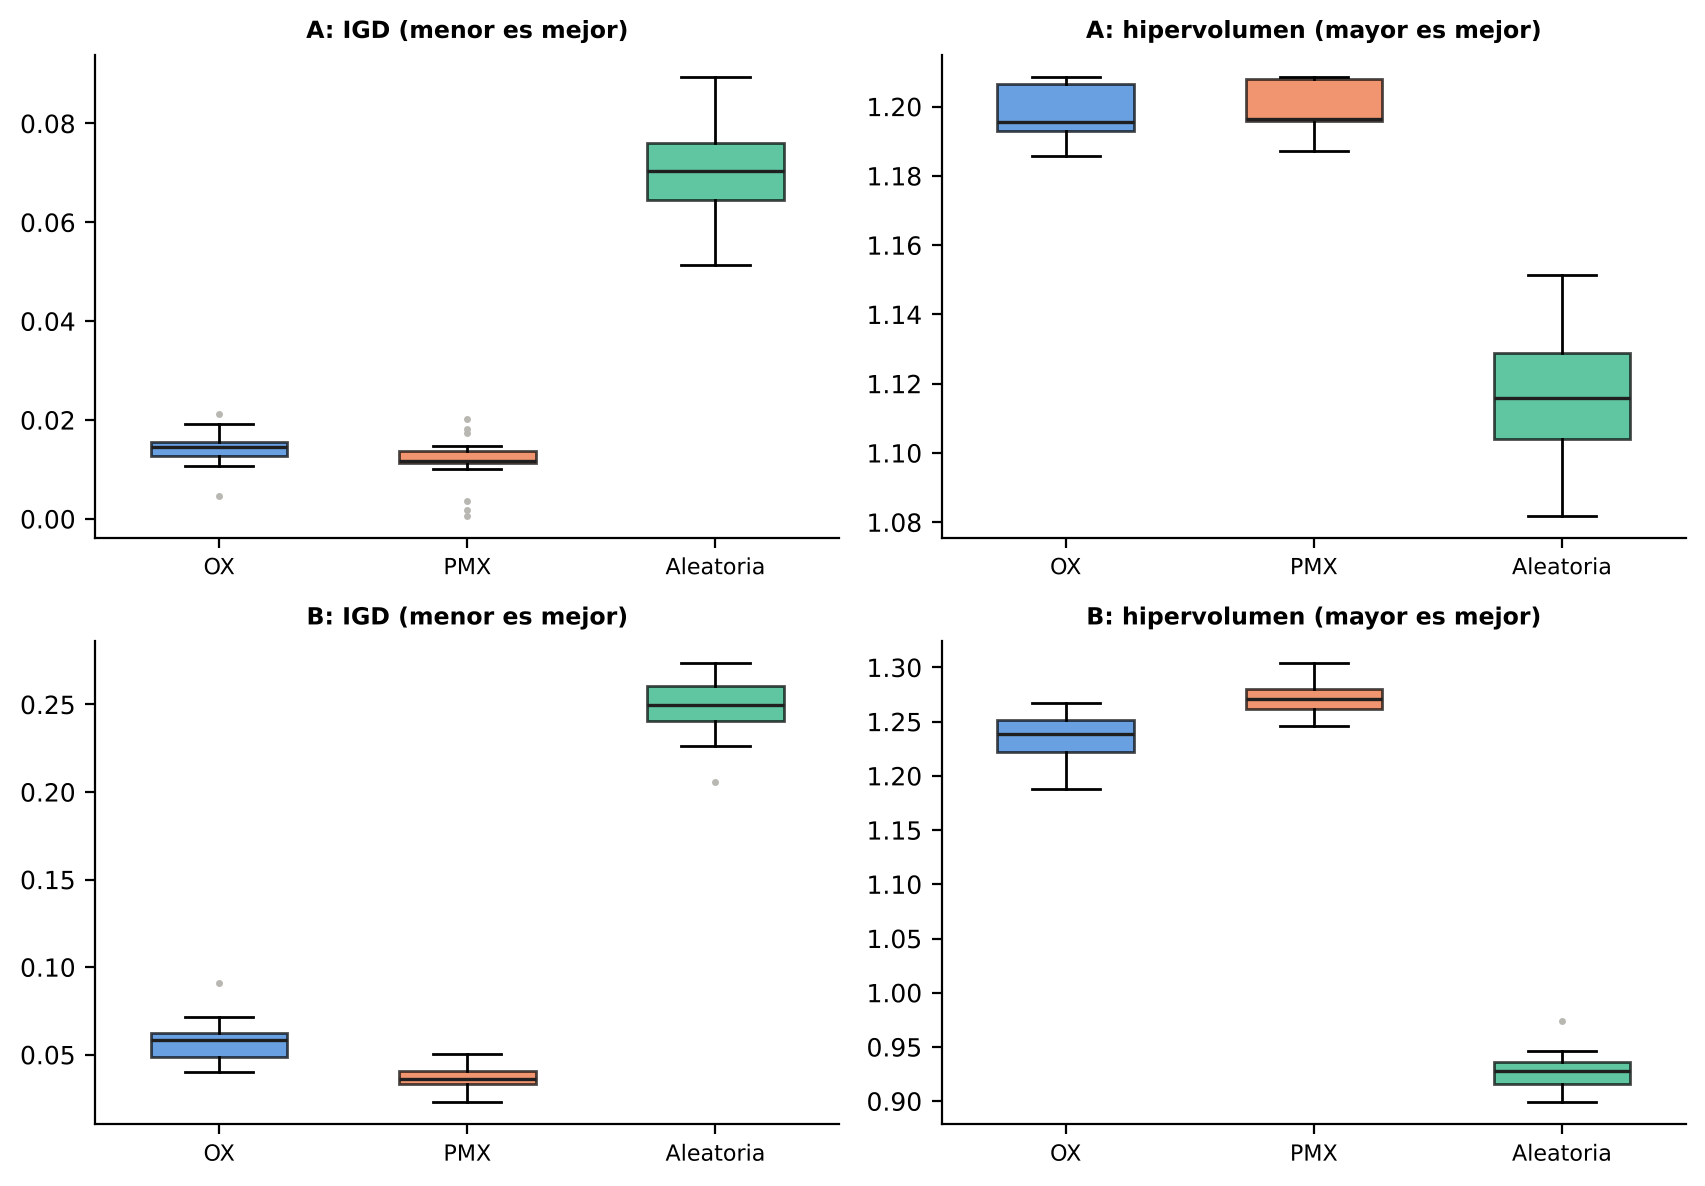
\includegraphics[width=0.9\linewidth]{../figuras/fig4_comparacion_metricas.png}
\caption{Distribución del IGD y del hipervolumen por algoritmo en las dos instancias (30 semillas).}
\label{fig:metricas}
\end{figure}

\section{Discusión}
Los resultados tienen tres lecturas. La primera es metodológica: la búsqueda aleatoria es inadecuada incluso en un espacio de 362\,880 secuencias, porque la mayor parte de las secuencias son de calidad media y la probabilidad de hallar un punto extremo del frente es muy baja. Un algoritmo que conserva y reproduce buenas subsecuencias encuentra en cambio la mayoría del frente con muy pocas evaluaciones.

La segunda es sobre los operadores. PMX produce mejores frentes que OX en ambas instancias. Una explicación plausible es que PMX preserva la posición absoluta de los lotes copiados, mientras que OX preserva su orden relativo; en un flow shop, la posición de un lote determina el tiempo en que llega a cada máquina, así que conservar posiciones puede ser más útil que conservar órdenes relativos. Este diagnóstico no fue verificado directamente y debe contrastarse con más instancias.

La tercera es para el decisor. El frente muestra que la secuencia de mínimo $C_{\max}$ no es la mejor para el cliente, porque su tardanza es elevada, y que la energía apenas cambia entre secuencias. El valor del modelo está en identificar secuencias de compromiso, como la de la Tabla~1, que mantienen el makespan casi óptimo y reducen la tardanza en más de la mitad. En la práctica, la elección final depende del costo relativo de una entrega tardía frente a un minuto de ciclo, algo que el decisor conoce y el algoritmo no.

\section{Limitaciones}
Los datos son sintéticos y calibrados con supuestos razonables, no con mediciones de planta; los conclusiones cuantitativas deben validarse con datos reales. La referencia de la instancia grande se construyó con los mismos algoritmos, lo que puede favorecerlos; por eso se reporta el número de puntos exactos recuperados solo para la instancia pequeña. La energía supone una política de apagado óptima con conocimiento de los huecos, que en la práctica requiere planeación de arranques. Por último, el estudio considera un solo tamaño de presupuesto por instancia y no incluye tiempos de alistamiento dependientes de la secuencia.

\section{Conclusiones}
Se formuló un flow shop de permutación con tres objetivos en conflicto: tiempo de terminación, tardanza ponderada y energía con dependencia de la secuencia. Para la instancia de nueve lotes, el frente exacto tiene 28 puntos, y NSGA-II con cruce PMX recupera en promedio 24 de ellos con 1.7\,\% de las evaluaciones posibles. PMX supera a OX en ambas instancias, y ambos operadores superan con claridad a la búsqueda aleatoria. Para la gestión de la producción, el resultado más útil es la existencia de secuencias de compromiso que reducen la tardanza en más de la mitad con un costo mínimo en $C_{\max}$ y energía, lo que justifica presentar al decisor el frente completo y no una única solución. El siguiente paso es validar el modelo con datos de una línea real y añadir tiempos de alistamiento dependientes de la secuencia.

\bibliographystyle{unsrtnat}
\bibliography{references}

\end{document}
